\documentclass[10pt,a4paper]{article}

\usepackage[margin=1in]{geometry}
\usepackage[T1]{fontenc}
\usepackage[utf8]{inputenc}
\usepackage{lmodern}
\usepackage{microtype}
\usepackage{graphicx}
\usepackage{booktabs}
\usepackage{tabularx}
\usepackage{array}
\usepackage{amsmath}
\usepackage{amssymb}
\usepackage{enumitem}
\usepackage{multirow}
\usepackage{xcolor}
\usepackage{subcaption}
\usepackage[numbers,sort&compress]{natbib}
\usepackage{hyperref}

\hypersetup{
  colorlinks=true,
  linkcolor=blue,
  citecolor=blue,
  urlcolor=blue
}

\newcommand{\best}[1]{\textbf{#1}}

\title{From Public Benchmarks to a Low-Resource Target Domain: A Comparative Study of Wood Surface Defect Detection}

\author{
  Khanh Nguyen-Trong$^{1,2}$\thanks{Corresponding author. Email: \texttt{khanhnt@ptit.edu.vn}}
}

\date{}

\begin{document}
\maketitle

\begin{center}
\small
$^{1}$ Intelligent Computing for Sustainable Development Lab, Posts and Telecommunications Institute of Technology (PTIT), Hanoi, Vietnam \\
$^{2}$ Faculty of Information Technology, Posts and Telecommunications Institute of Technology (PTIT), Hanoi, Vietnam
\end{center}

\begin{abstract}
This study investigates wood surface defect detection across three practically important settings: a curated public-benchmark protocol, a broader in-domain seven-class protocol, and transfer to a low-resource target domain. We compare lightweight Faster R-CNN + MobileNetV3-FPN detectors, a compact YOLOv8s baseline, and two small-object-oriented YOLO variants across those settings. Across the in-domain experiments, detector family matters more than the local YOLO refinements tested here. In the matched 50-epoch screening runs, YOLOv8s stays ahead of the MobileNet-based two-stage baselines, whose best AP50 values are 74.52\% on the curated benchmark and 75.15\% on the broader seven-class protocol. The long-schedule YOLOv8s run on the curated benchmark reaches 84.38\% AP50, which places it toward the upper end of the values reported in recent public studies built on the same public benchmark domain. The broader seven-class protocol remains harder, with both the 50-epoch and 200-epoch references remaining below the final curated-benchmark result. Repeated-seed 50-epoch checks do not overturn the curated-benchmark ordering, and the matched 200-epoch reruns of the P2-head and WNIoU-style variants remain below the final curated-benchmark baseline, with \texttt{Y1-e200} and \texttt{Y2-e200} reaching 83.70\% and 83.93\% AP50, respectively.

For external transfer, the picture is more mixed. On VNWoodKnot, source initialization improves optimization speed and yields a stronger representative seed-42 run, but the four-seed held-out-test aggregate does not confirm a robust AP50 advantage over target-only training under the same 50-epoch budget. Overall, benchmark curation, evaluation protocol, and dataset shift shape the observed ranking almost as much as detector design itself.
\end{abstract}

\noindent\textbf{Keywords:} wood surface defect detection; lightweight detector comparison; MobileNetV3-FPN; YOLOv8; benchmark sensitivity; industrial visual inspection; domain shift

\section{Introduction}
\label{sec:introduction}

Automatic surface inspection is a persistent requirement in industrial production because manual inspection is costly, subjective, and difficult to scale. In wood processing, the problem is even harder than in many manufactured materials because the substrate is inherently heterogeneous: grain, resin, knots, cracks, pith, stains, and growth patterns create large appearance variation even before true defects are considered. This challenge belongs to a broader wood-vision research landscape that spans species recognition, texture analysis, grading, and material characterization, where strong appearance variability, limited labeled data, and domain-specific acquisition settings have long been recognized as central obstacles \citep{hwang_sugiyama_review,da_silva_2017,souza_2020,de_geus_2021,kirbas_2022,he_2021_woodresearch,herrera_poyatos_2024}. Kodytek \textit{et al.} note that surface defects do not merely lower visual quality; they can also degrade strength and stiffness, which directly affects material utilization and economic value in downstream processing \citep{kodytek_dataset}. In practice, an inspection system must therefore detect visually weak defects, separate semantically similar subtypes, and remain stable across production batches while using detector choices that are realistic for deployment rather than only optimal on a curated benchmark.

The defect types themselves are also operationally meaningful. Several common categories were presented in the literature, including live knots, dead knots, quartzity, knots with cracks, missing knots, cracks, overgrown regions, resin, marrow, and blue stain \citep{kodytek_dataset}. A live knot usually corresponds to a branch remnant that remains relatively intergrown with surrounding fibers, whereas a dead knot is more detached and may indicate weaker local structure or later breakout during machining. A knot with crack combines fiber distortion with fracture-like splitting, and a missing knot leaves a cavity or void that directly reduces usable surface quality. Longitudinal cracks can propagate during drying, handling, or cutting. Resin creates contamination and finishing problems, marrow often lowers appearance grade and dimensional stability, and blue stain reduces commercial value even when the mechanical damage is less obvious. In this study, we focus on seven frequent and practically important defect classes: live knot, dead knot, knot with crack, knot missing, crack, resin, and marrow. 

From a vision perspective, wood surface defect detection is challenging for several reasons. First, many targets are small relative to the board image and may appear low-contrast, elongated, or only partially visible, which makes localization unstable under repeated downsampling. Second, several categories such as live knots, dead knots, knots with cracks, and cracks are semantically close and visually entangled, so subtype confusion is easy even when a detector fires near the right region. Third, the class distribution is long-tailed, which makes rare but operationally meaningful defects hard to learn. Fourth, deployment data rarely match benchmark data in framing, scale, label taxonomy, or defect prevalence, so transfer behavior matters as much as in-domain validation.

Most recent work responds to these difficulties by redesigning the detector. Representative wood-defect models include ODCA-YOLO \citep{odca_yolo}, BPN-YOLO \citep{bpn_yolo}, SiM-YOLO \citep{sim_yolo}, FDD-YOLO \citep{fdd_yolo}, and CWB-YOLOv8 \citep{an_cwb_yolov8}. Related wood-inspection studies have also explored anomaly-oriented detection and hybrid sensing setups \citep{kilic_2024,kilic_2025_wd_detector}. Similar priorities appear in recent inspection work on faulty wood regions, small industrial defects, PCB faults, rail defects, and metallic or steel surfaces \citep{cmc_wood_area_attention,cmc_insulator_small,cmc_pcb_yolov8,cmc_cg_yolov8,cmc_rail_upernet,cmc_yolo_rlc,cmc_lmvit,cmc_msese,cmc_flame,cmc_channel_shuffle}. Across these papers, the same trade-offs keep resurfacing: small targets disappear at coarse scales, localization is fragile on weak or elongated defects, and the detector still has to fit a practical compute budget.


Beyond curated benchmark performance, it remains unclear whether detector rankings remain stable when evaluation protocols are broadened or when models are transferred to lower-resource target domains. This question is practically relevant in settings where labeled wood-defect data are limited, including emerging local datasets such as VNWoodKnot. For that reason, we are interested not only in which detector performs best on the public benchmark domain, but also in how well knowledge learned from larger wood-defect datasets transfers to a local setting with much less data. In practical terms, this raises three questions. Do strong results on the curated benchmark still hold when the evaluation protocol is broadened? Does detector family matter more than a small module-level refinement? And when the model is moved to a different dataset, how much performance is lost as label space, framing, and object scale change?

Given practical compute constraints, we focus on lightweight models: Faster R-CNN with MobileNetV3-FPN, a compact YOLOv8s baseline, and two small-object-oriented YOLO variants with a P2 head and a custom WNIoU-style hybrid box loss. We study them on two datasets: the public benchmark domain \citep{kodytek_dataset} and VNWoodKnot, a smaller and low-resource dataset collected in Vietnam \citep{TRAN2025112039}. The goal is straightforward: to see which conclusions still hold once benchmark accuracy is no longer the only thing that matters.

This study makes the following contributions.

\begin{enumerate}[leftmargin=1.5em]
  \item We present a comparative evaluation spanning a curated public-benchmark protocol, a broader in-domain seven-class protocol, and a low-resource target-domain setting.
  \item We compare lightweight two-stage detectors and a compact one-stage detector family under shared processing and evaluation conditions.
  \item We show that benchmark breadth materially affects apparent detector performance under the studied protocols.
    \item We distinguish single-run and repeated-seed transfer behavior on VNWoodKnot under a fixed fine-tuning budget.
\end{enumerate}

The rest of the paper is organized as follows. Section~\ref{sec:related-work} reviews prior work on wood defect detection, detector design, and evaluation practice. Section~\ref{sec:methods} describes the datasets, protocol variants, detector configurations, training setup, and evaluation protocol. Section~\ref{sec:experiments} presents the experimental scenarios and results, covering detector-family comparison, focused YOLO analysis, and target-domain adaptation on VNWoodKnot. Section~\ref{sec:discussion} discusses the main findings in terms of benchmark sensitivity, detector choice, and transfer behavior. Finally, Section~\ref{sec:conclusion} concludes the paper and outlines possible directions for future work.

\section{Related Work}
\label{sec:related-work}

%\subsection{Wood Defect Detection on Curated Benchmarks}

Recent works on wood defect detection commonly evaluate YOLO-style detectors on benchmark variants derived from the public benchmark domain, including ODCA-YOLO, BPN-YOLO, SiM-YOLO, FDD-YOLO, and CWB-YOLOv8 \citep{odca_yolo,bpn_yolo,sim_yolo,fdd_yolo,an_cwb_yolov8}. Although these models differ in where they add capacity, the overall recipe is similar: they retain a one-stage backbone and then introduce feature fusion, attention, small-target handling, or a modified localization loss to improve the reported score. The large-scale image dataset of wood surface defects introduced by Kodytek \textit{et al.}, which we refer to here as the VSB dataset, has become the common reference point for this line of work because it offers a clearer taxonomy and a more systematic benchmark than many earlier in-house collections \citep{kodytek_dataset}.

Wood inspection research is broader than bounding-box detection, however. Kilic \textit{et al.} \citep{kilic_2024,kilic_2025_wd_detector} study anomaly-oriented and hybrid sensing settings, and Hoang \textit{et al.} \citep{cmc_wood_area_attention} report 60.6\% AP and 81.2\% AP50 for an area-attention detector on a relabeled benchmark variant built from the Kodytek dataset, but with a relabeling scheme different from the original VSB taxonomy. Their method also exceeds the YOLOv12 reference reported in the same paper, which reaches 55.3\% AP and 74.3\% AP50. This is a useful neighboring reference because it is built from the same image source but uses a different label definition and evaluation framing. More broadly, it shows that wood inspection is still evaluated under multiple benchmark variants rather than under one universally accepted setup. Even within detector papers, the result format is usually the same: one curated split, one headline AP50, and one proposed architectural change. That convention makes the literature easy to scan, but it leaves open a practical question that matters to deployment: is the reported gain attached to the detector itself, or to the way the benchmark was screened and measured?

%\subsection{Detector Choice Under Practical Constraints}

The broader industrial-inspection literature looks at the same problem from a slightly different angle. Reviews of edge-oriented and industrial defect detection put latency, memory footprint, and backbone efficiency on the same footing as accuracy \citep{mittal_2024,ma_2024_air,wang_2025_ieeeaccess}. That is one reason two-stage detectors such as Faster R-CNN remain useful as controlled references, especially when paired with lightweight backbones such as MobileNetV3 \citep{faster_rcnn,mobilenetv3}. At the same time, YOLO-style one-stage detectors have become the practical default in many inspection tasks because they offer dense prediction with a favorable speed--accuracy trade-off.

The same trade-off shows up in compact detectors for PCB, aluminum, printed-surface, metallic, rail, and steel inspection, where authors repeatedly return to the same toolbox: lighter backbones, efficient heads, multiscale fusion, and revised box losses \citep{cmc_pcb_yolov8,cmc_yolo_rlc,cmc_cg_yolov8,cmc_aluminum_yolov8n,cmc_printed_positive,cmc_channel_shuffle,cmc_insulator_small,cmc_msese,cmc_rail_upernet}. Small-object surveys tell a similar story. High-resolution heads and alternative localization losses are standard responses when targets are small, weakly contrasted, or easy to miss after repeated downsampling \citep{wei_2024_smallreview,hua_2025_smallsurvey}. That background is exactly why our study keeps both ingredients in view: detector-family choice and small-object-oriented YOLO refinements.

%\subsection{Protocol Breadth, Reproducibility, and Transfer}

Cross-paper detector results are still hard to compare cleanly. Reviews and benchmarking papers keep making the same point: datasets, split rules, and metrics are not reported in a fully consistent way, so cross-paper ranking can look firmer than it really is \citep{fdd_yolo,ma_2024_air,wang_2025_ieeeaccess}. In wood inspection, that matters immediately. Changing class filters, screening rules, or sampling policy can change which model looks best. A detector that performs well on a small curated subset may not keep the same advantage once the protocol is broadened, and neither result says much by itself about transfer to a different dataset. That is the point of departure for our study. We keep the detector set compact and ask two practical follow-up questions: what still holds when the source-domain protocol is broadened, and what still holds when the model is moved to VNWoodKnot?

\section{Materials and Methods}
\label{sec:methods}

%\subsection{Datasets and Protocol Variants}
\subsection{Datasets and Protocol Design}
\label{sec:datasets}

In this study, we use the VSB-derived source as the public benchmark domain for both the curated benchmark and the broader seven-class protocol, whereas VNWoodKnot is used as the external target domain for adaptation experiments. The in-domain experiments are built on the large-scale wood surface defect dataset of Kodytek \textit{et al.} \citep{kodytek_dataset}. Similarly to previous studies on this dataset, we derive a seven-class label space consisting of \texttt{live\_knot}, \texttt{dead\_knot}, \texttt{resin}, \texttt{knot\_with\_crack}, \texttt{crack}, \texttt{marrow}, and \texttt{knot\_missing}. This shared label space is used for both the curated benchmark and the broader seven-class protocol so that protocol sensitivity can be analyzed without changing the task definition.


\begin{figure*}[t]
  \centering
  \begin{subfigure}[t]{0.48\textwidth}
    \centering
    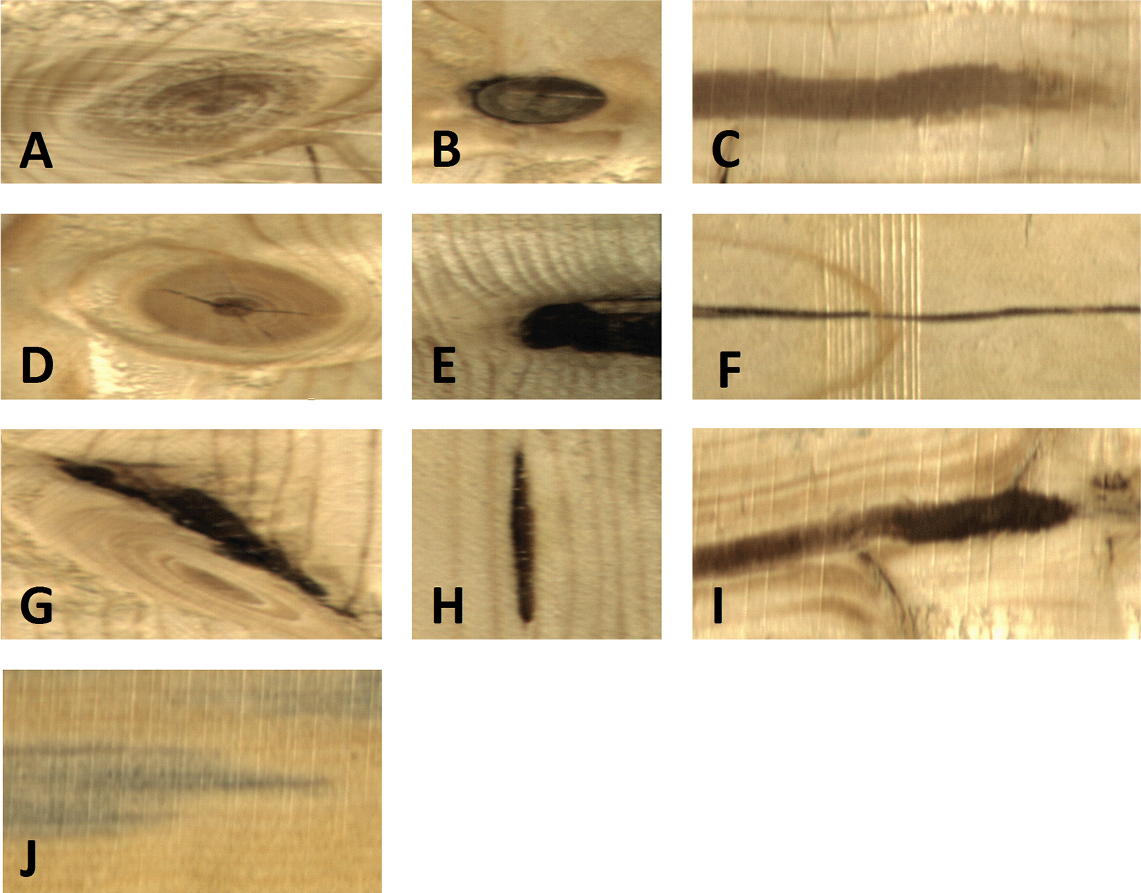
\includegraphics[width=\linewidth]{figures/wood_defect_types.png}
    \caption{Representative defect categories from the public benchmark domain. The original dataset includes ten defect types, from which the seven-class protocol used in this study is derived \citep{kodytek_dataset}.}
    \label{fig:dataset-overview-public}
  \end{subfigure}\hfill
  \begin{subfigure}[t]{0.48\textwidth}
    \centering
    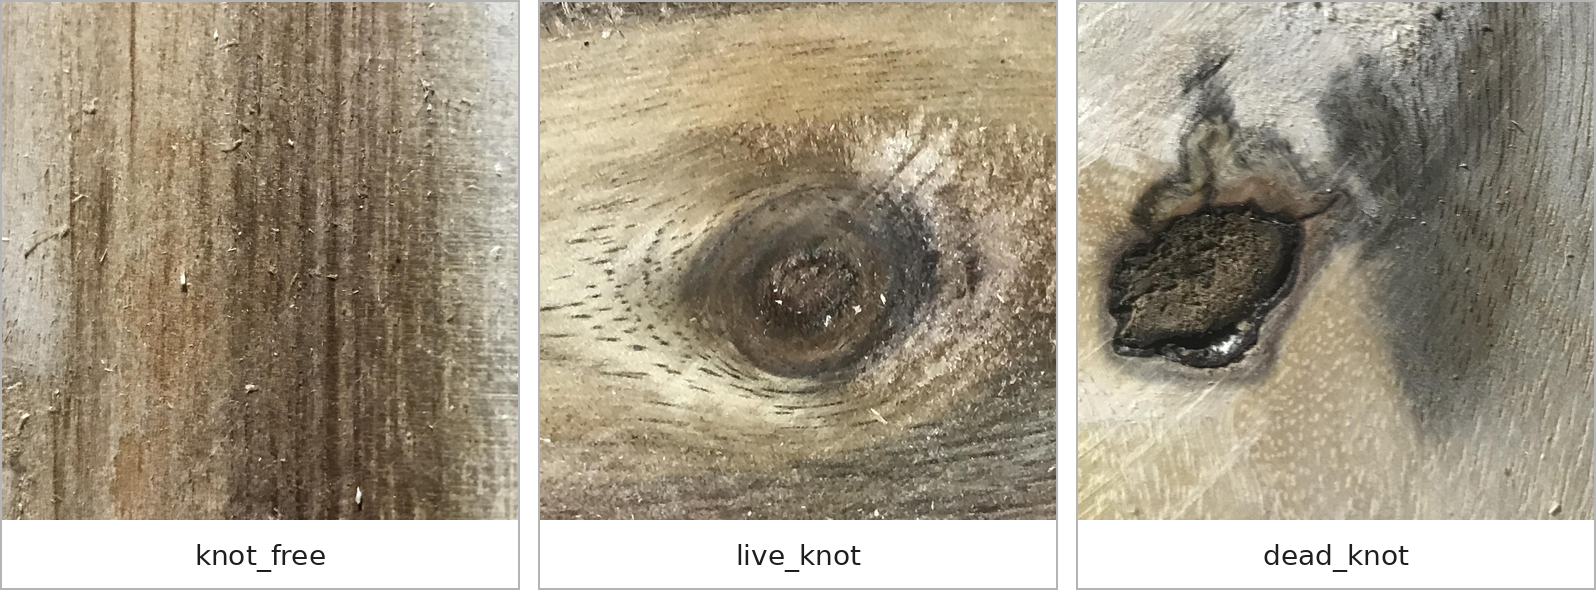
\includegraphics[width=\linewidth]{figures/vnwoodknot_triptych.png}
    \caption{Representative images from VNWoodKnot, showing the three labels available in the original dataset: \texttt{knot\_free}, \texttt{live\_knot}, and \texttt{dead\_knot} \citep{TRAN2025112039}.}
    \label{fig:dataset-overview-vn}
  \end{subfigure}
  \caption{Visual comparison of the two datasets used in this study. The left panel represents the public benchmark domain used to construct the curated benchmark and the broader seven-class protocol, while the right panel shows the low-resource target domain used for supervised adaptation experiments. The contrast in defect scale, framing, and label structure is one of the central motivations for the comparative evaluation.}
  \label{fig:dataset-overview}
\end{figure*}



%\paragraph{Low-resource target domain: VNWoodKnot.}
To reflect that Vietnamese local setting, we use VNWoodKnot  \citep{TRAN2025112039}, a recent dataset collected in Vietnam for wood knot detection and classification. It consists of board-surface images acquired under a fixed local imaging setup and annotated around knot-related categories, making it a useful low-resource target domain for this study. The original VNWoodKnot label space contains \texttt{knot\_free}, \texttt{live\_knot}, and \texttt{dead\_knot}. In our study, the two knot classes form the detection task, while \texttt{knot\_free} images are preserved as negative samples. This makes VNWoodKnot a practically relevant low-resource target domain for evaluating supervised adaptation rather than a direct seven-class benchmark.

%\subsection{Dataset Analysis and Domain Shift Indicators}
%\label{sec:data-analysis}

Figure~\ref{fig:dataset-overview} gives a visual comparison, while Table~\ref{tab:dataset-comparison} summarizes the main quantitative differences between the two datasets. These differences matter because the public benchmark domain mainly tests small-defect localization under a richer seven-class taxonomy, whereas the target domain emphasizes larger knots under a much smaller label space.

\begin{table*}[t]
  \centering
  \caption{Comparison between the public benchmark domain and the low-resource target domain used in this study.}
  \label{tab:dataset-comparison}
  \footnotesize
  \setlength{\tabcolsep}{5pt}
  \begin{tabularx}{0.94\textwidth}{>{\raggedright\arraybackslash}p{0.24\textwidth} >{\raggedright\arraybackslash}X >{\raggedright\arraybackslash}X}
    \toprule
    Attribute & Public benchmark domain (VSB-derived) & Low-resource target domain (VNWoodKnot) \\
    \midrule
    Role in this study & Source benchmark for in-domain comparison, protocol-sensitivity analysis, and source pretraining & External target domain for supervised adaptation under limited data \\
    Source images & 20,276 & 1,515 \\
    Box annotations & 43,974 & 1,021 \\
    Label space used in this study & 7 classes: \texttt{live\_knot}, \texttt{dead\_knot}, \texttt{resin}, \texttt{knot\_with\_crack}, \texttt{crack}, \texttt{marrow}, \texttt{knot\_missing} & 2 detection classes (\texttt{live\_knot}, \texttt{dead\_knot}) with \texttt{knot\_free} retained as negatives \\
    Image format & Heterogeneous source images converted into tiled training/evaluation records & Fixed-size images ($1500 \times 1500$) \\
    Derived tiles / processed images & 48,156 tiles after preprocessing (38,493 train / 4,879 val / 4,784 test) & No tiling used in the reported target-domain setting \\
    Reported split sizes & 38,493 / 4,879 / 4,784 tiles (train / val / test) & 1,060 / 226 / 229 images and 715 / 151 / 155 boxes (train / val / test) \\
    Empty / background-only images & Not emphasized in the benchmark protocol & 500 \texttt{knot\_free} images \\
    %Mean normalized bbox area & 0.008857 & 0.119985 \\
    %Small-annotation ratio & 75.95\% (33,400 / 43,974) & 0\% (0 / 1,021) under the same rule \\
    Main implication & Strong emphasis on small-defect localization and long-tail multi-class discrimination & Stronger emphasis on larger knot regions, simpler label space, and source-to-target transfer \\
    \bottomrule
  \end{tabularx}
\end{table*}

%\paragraph{In-domain dataset size and tiling.}
The in-domain dataset audit reports 20,276 source images and 43,974 box annotations. Under the tiling pipeline used in this study, these source images yield 48,156 tile images, with 38,493 train / 4,879 validation / 4,784 test tiles. This tile-based protocol is the basis for all in-domain training and evaluation.

%\paragraph{Small-defect prevalence (in-domain vs external).}
Small objects dominate the in-domain dataset: 33,400 out of 43,974 annotations (75.95\%) satisfy the same small-defect rule used in our evaluation summaries. In contrast, VNWoodKnot has effectively zero small annotations under that rule (0 out of 1,021). This implies that the in-domain task is heavily influenced by small-defect localization, whereas VNWoodKnot emphasizes larger knot boxes.

%\paragraph{Bounding-box scale mismatch.}
The mean normalized bounding-box area in the in-domain dataset is 0.008857, whereas VNWoodKnot has a mean normalized bounding-box area of 0.119985. This order-of-magnitude gap indicates a strong difference in object scale and framing. Together with the label-space reduction and the presence of many negative images in VNWoodKnot, these statistics support interpreting the external evaluation as a substantial source-to-target shift rather than as a minor threshold-calibration issue.

\subsection{Protocol Variants}
\label{sec:protocol}

\subsubsection{Protocol A: Curated seven-class benchmark}
We define the curated benchmark to be comparable in spirit to prior seven-class benchmark variants derived from the Kodytek dataset \citep{kodytek_dataset}. Following prior studies \citep{odca_yolo,bpn_yolo,sim_yolo,fdd_yolo,an_cwb_yolov8}, we first select 3,600 source images and assign train, validation, and test splits at the source-image level before generating tiled records for detection training and evaluation. All tiles derived from the same source image therefore remain in the same split. This benchmark contains 7,679 training tiles, 977 validation tiles, and 972 test tiles. For experiments on this protocol, we retain short-budget 50-epoch runs for detector screening and ablation, and we also include a 200-epoch run as the literature-facing confirmation schedule.

\subsubsection{Protocol B: Full seven-class protocol}
To check whether conclusions from the curated benchmark remain valid under the broader seven-class protocol, we also evaluate a full seven-class protocol constructed by filtering the full dataset down to the same seven classes. This protocol produces a larger validation split with 4,846 validation tiles under the present tiling configuration. As in Protocol A, we keep the original 50-epoch run as the short-budget reference, and we also include a 200-epoch YOLO run to better match the longer schedules commonly used in prior YOLO-based studies.

\subsubsection{External protocol: VNWoodKnot adaptation setting}
For the external study, VNWoodKnot is reformulated as a two-class detection task containing \texttt{live\_knot} and \texttt{dead\_knot}, while \texttt{knot\_free} images are preserved as negatives. This setting allows us to measure how quickly a curated-benchmark source checkpoint can adapt to a target wood-inspection dataset under a fixed fine-tuning budget.



\subsection{Detector Variants}
\label{sec:detectors}

Based on the defect characteristics discussed in Sections~\ref{sec:introduction} and \ref{sec:datasets}, we select three detector families to cover complementary operating points in a practical wood-inspection design space. First, Faster R-CNN with MobileNetV3-FPN provides a proposal-based two-stage family that combines explicit region refinement with lightweight backbones, making it a relevant reference when localization control and computational efficiency must be balanced \citep{faster_rcnn,mobilenetv3,mittal_2024}. Second, YOLOv8s represents a compact one-stage family that has become a strong practical default in recent defect-inspection and wood-defect studies because of its favorable speed--accuracy trade-off and multiscale dense prediction behavior \citep{odca_yolo,bpn_yolo,sim_yolo,fdd_yolo}. Third, we test two targeted YOLO refinements, namely a higher-resolution P2 head and a custom WNIoU-style hybrid box loss. The latter combines a CIoU term, an NWD-like similarity term, and a Wise-IoU-style focusing factor to test whether more robust localization supervision helps thin cracks and irregular knot-related regions \citep{tong_2023_wiseiou,wang_2021_nwd,zheng_2020_diou}. This detector selection allows the study to address two practical questions at once: which detector family is most suitable for the present wood-defect setting, and whether widely motivated small-object-oriented refinements materially change that ranking.


\subsubsection{Low-capacity MobileNet baseline}
The lowest-capacity reference in our study is a Faster R-CNN detector instantiated from Faster R-CNN + MobileNetV3-320-FPN,  with the image size fixed to $1024 \times 1024$. We include this model as a lower-cost anchor point for the proposal-based family, so that the study can distinguish between the effect of detector family and the effect of simply scaling backbone capacity inside the same two-stage design \citep{faster_rcnn,mobilenetv3}.

\subsubsection{High-resolution MobileNet baseline}
The main lightweight family in the paper uses Faster R-CNN + MobileNetV3-Large-FPN, trained at $1024 \times 1024$. This family appears in one broader-protocol run and several curated-benchmark variants summarized later in the experiment tables. We use it as the principal lightweight two-stage reference because it retains the proposal-based refinement behavior of Faster R-CNN while providing a stronger MobileNet backbone than the lower-capacity baseline above \citep{faster_rcnn,mobilenetv3}.

\subsubsection{YOLOv8s baseline (Y0)}
The YOLOv8s runs on the broader seven-class protocol and on the curated benchmark use the standard YOLOv8s architecture. We choose this network as the compact one-stage baseline because it provides a modern, strong, and deployment-relevant detector family that is close in spirit to the YOLO-style models dominating recent wood-defect literature \citep{odca_yolo,bpn_yolo,sim_yolo,fdd_yolo}. The final reported run on the curated benchmark is denoted \texttt{Y0-3600e200}.

\subsubsection{P2-head ablation (Y1)}
\texttt{Y1} adds an extra P2 detection head to YOLOv8s via a modified model configuration. This variant is motivated by a task-specific hypothesis: several wood defects in the present benchmark occupy small image regions or exhibit weak local contrast, so discriminative cues may be attenuated when prediction begins only from coarser pyramid levels. In feature-pyramid notation, the baseline YOLOv8s branch predicts from $\{P_3, P_4, P_5\}$, whereas \texttt{Y1} extends this set to $\{P_2, P_3, P_4, P_5\}$. Adding a higher-resolution detection layer therefore tests whether earlier multiscale prediction improves the representation of small defects in this domain, as suggested by recent small-object detection studies \citep{wei_2024_smallreview,hua_2025_smallsurvey,cmc_insulator_small}. In the present study, \texttt{Y1} is examined first as a 50-epoch screening-stage ablation and then as a matched 200-epoch comparison on the curated benchmark.

\subsubsection{WNIoU-style box-loss ablation (Y2)}
\texttt{Y2} modifies the box regression loss to a custom WNIoU-style hybrid loss. In our implementation, this loss combines a CIoU term, an NWD-like similarity term, and a Wise-IoU-style focusing factor, rather than reproducing a single published formula verbatim \citep{tong_2023_wiseiou,wang_2021_nwd,zheng_2020_diou}. This variant addresses a different hypothesis from \texttt{Y1}: some wood defects, particularly thin cracks and irregular knot-related regions, may be limited less by feature resolution than by unstable geometric supervision during box regression. A distance-aware and reweighted localization loss is therefore tested as a compact way to improve localization robustness without modifying the detector architecture itself. In the comparison reported here, \texttt{Y2} appears as a matched 200-epoch curated-benchmark rerun under the same long schedule as the final compact baseline.

For the YOLO branch, we write the detection objective as
\begin{equation}
\mathcal{L}_{\text{det}} = \mathcal{L}_{\text{cls}} + \mathcal{L}_{\text{dfl}} + \mathcal{L}_{\text{box}}.
\end{equation}
The baseline YOLOv8s and the P2-head variant keep the standard CIoU-based box term,
\begin{equation}
\mathrm{CIoU} = \mathrm{IoU} - \frac{\rho^2(\mathbf{b}, \mathbf{b}^{\ast})}{c^2} - \alpha_{\mathrm{ciou}} v,
\end{equation}
where $\mathbf{b}$ and $\mathbf{b}^{\ast}$ are the predicted and target boxes, $\rho^2(\cdot,\cdot)$ is the squared center distance, $c$ is the diagonal length of the smallest enclosing box, and $v$ is the aspect-ratio consistency term \citep{zheng_2020_diou}. For \texttt{Y2}, we replace $\mathcal{L}_{\text{box}}$ with a hybrid form. First, an NWD-style similarity is computed on normalized boxes,
\begin{equation}
S_{\mathrm{nwd}} = \exp\!\left(
-\frac{
\sqrt{
(c_x-c_x^{\ast})^2 + (c_y-c_y^{\ast})^2 +
\frac{1}{4}\left[(w-w^{\ast})^2 + (h-h^{\ast})^2\right]
}
}{s}
\right),
\end{equation}
where $(c_x, c_y, w, h)$ and $(c_x^{\ast}, c_y^{\ast}, w^{\ast}, h^{\ast})$ denote predicted and target box centers and sizes, and $s$ is a distance scale (set to $0.05$ in this study). We then form the blended base loss
\begin{equation}
\mathcal{L}_{\text{base}} = (1-\lambda)(1-\mathrm{CIoU}) + \lambda(1-S_{\mathrm{nwd}}),
\end{equation}
with $\lambda = 0.30$, and apply a Wise-IoU-style difficulty weight
\begin{equation}
w_{\mathrm{focus}} = 1 + \beta (1-\mathrm{CIoU})^{\gamma},
\end{equation}
with $\beta = 0.50$ and $\gamma = 1.00$. The final custom box term is therefore
\begin{equation}
\mathcal{L}_{\text{box}}^{\texttt{Y2}} = w_{\mathrm{focus}} \, \mathcal{L}_{\text{base}}.
\end{equation}
This design preserves the original YOLOv8 classification and distribution-focal terms while changing only the localization supervision.


\begin{table}[t]
  \centering
  \caption{Detector families covered in the study.}
  \label{tab:detector-families}
  \footnotesize
  \setlength{\tabcolsep}{4pt}
  \begin{tabularx}{\linewidth}{>{\raggedright\arraybackslash}p{0.16\linewidth} >{\raggedright\arraybackslash}p{0.28\linewidth} >{\raggedright\arraybackslash}p{0.23\linewidth} X}
    \toprule
    Family & Implementation & Experiments & Role in study \\
    \midrule
    MobileNet-low & Faster R-CNN + MobileNetV3-320-FPN & \texttt{baseline\_detector} & exploratory low-capacity reference \\
    MobileNet-HR & Faster R-CNN + MobileNetV3-Large-FPN & \texttt{B1}, \texttt{E1} & lightweight high-resolution baseline family \\
    YOLO baseline & YOLOv8s & \texttt{Y0-full}, \texttt{Y0-full\_e200}, \texttt{Y0-3600e200} & compact one-stage main baseline \\
    YOLO refinement & YOLOv8s + P2 / WNIoU & \texttt{Y1}, \texttt{Y1-e200}, \texttt{Y2-e200} & targeted ablations \\
    \bottomrule
  \end{tabularx}
\end{table}



\section{Experiments and Results}
\label{sec:experiments}

\subsection{Training Setup and Evaluation Settings}
\label{sec:training}

\subsubsection{Hyperparameters and metrics}
We use a shared YOLO training setup wherever possible, including image size $1024$, mixed-precision training, AdamW as the optimizer, and training seed 42. The experiments are organized in two stages. First, we use a 50-epoch budget for detector-family comparison and short-budget ablation analysis inside the study. Second, we extend the curated-benchmark YOLO branch to 200 epochs to test whether the short-budget ranking remains stable under a longer schedule. This long-schedule stage includes the final compact baseline (\texttt{Y0-3600e200}) together with matched 200-epoch reruns of the P2 and WNIoU variants (\texttt{Y1-e200} and \texttt{Y2-e200}). The broader seven-class protocol is also rerun for 200 epochs as a schedule diagnostic.

All models are trained and evaluated under a consistent export and evaluation pipeline. For VNWoodKnot adaptation, both runs (\texttt{T0} and \texttt{T1}) use the same two-class target-domain split and are evaluated on the held-out target-domain test set with the same evaluator.

To stay comparable with recent YOLO-based wood-defect studies, we use AP50 as the primary metric. We also report precision and recall at IoU 0.5 (denoted Prec.50 and Rec.50), with
\begin{equation}
\mathrm{Prec.50} = \frac{TP}{TP + FP},
\qquad
\mathrm{Rec.50} = \frac{TP}{TP + FN},
\end{equation}
and we interpret AP50 as the area under the precision--recall curve at IoU $\geq 0.5$,
\begin{equation}
\mathrm{AP50} = \int_{0}^{1} \mathrm{Prec.50}(R)\, dR.
\end{equation}
In addition, we monitor a small-target subset metric for in-domain evaluation. Under the rule used in the dataset audit and evaluator, an annotation is treated as small if its normalized bounding-box area is $\leq 0.01$, or its width is $\leq 16$ pixels, or its height is $\leq 16$ pixels, with \texttt{combine=any}. These auxiliary values are reported for completeness but are not emphasized in the main result tables.

For VNWoodKnot, the external comparison is a supervised two-class target-domain evaluation. The two classes are \texttt{live\_knot} and \texttt{dead\_knot}, while \texttt{knot\_free} images are preserved as negative samples. This makes the external study a matched adaptation problem rather than an overlap-only label-mapping exercise.

\subsubsection{Experiment scenarios}

We evaluate four scenarios.
\begin{itemize}
\item Detector-family exploration (\texttt{B1}, \texttt{E1}): We compare lightweight Faster R-CNN + MobileNet baselines and compact YOLO baselines to identify a practical detector family before testing local YOLO refinements.

\item Curated benchmark (\texttt{Y0-3600}, \texttt{Y0-3600e200}, \texttt{Y1}, \texttt{Y1-e200}, \texttt{Y2-e200}): Train and evaluate on the curated benchmark using \texttt{Y0-3600} as the short-budget reference and \texttt{Y0-3600e200} as the final literature-facing confirmation run. The P2 variant is reported both as a 50-epoch screening-stage comparison and as a matched 200-epoch rerun, whereas the WNIoU-style loss variant is included as a matched 200-epoch rerun under the same curated-benchmark protocol.

\item Broader seven-class protocol (\texttt{Y0-full}, \texttt{Y0-full\_e200}): Train and evaluate on the broader seven-class protocol to quantify the protocol-sensitivity gap relative to the curated benchmark. We retain the original 50-epoch checkpoint as the stronger study-internal reference, and we use an additional 200-epoch rerun as a diagnostic check on schedule sensitivity.

\item Target domain adaptation (\texttt{T0}, \texttt{T1}): Compare supervised target-only training (\texttt{T0}) and curated-benchmark source fine-tuning (\texttt{T1}) on the VNWoodKnot two-class protocol. Both runs are trained for 50 epochs and then evaluated on the held-out target-domain test split. The validation trajectories over the same 50-epoch budget are reported as optimization diagnostics.
\end{itemize}

Table~\ref{tab:experiment-summary} summarizes the main runs reported in the manuscript and the role each one plays in the study.

\begin{table*}[t]
  \centering
  \caption{Summary of the experiments}
  \label{tab:experiment-summary}
  \scriptsize
  \setlength{\tabcolsep}{4pt}
  \begin{tabularx}{\textwidth}{>{\raggedright\arraybackslash}p{0.12\textwidth} >{\raggedright\arraybackslash}p{0.23\textwidth} >{\raggedright\arraybackslash}p{0.17\textwidth} c X}
    \toprule
    ID & Model / Change & Protocol & Epochs & Description \\
    \midrule
    \texttt{B1} & Faster R-CNN + high-resolution MobileNet & Full seven-class & 50 & Primary lightweight two-stage reference for the broader seven-class protocol. \\
    \texttt{E1} & Faster R-CNN + high-resolution MobileNet & Curated benchmark & 50 & Primary lightweight two-stage reference for the curated benchmark. \\
    \texttt{Y0-3600} & YOLOv8s & Curated benchmark & 50 & Main short-budget curated-benchmark reference used in the focused YOLO comparison. \\
    \texttt{Y0-3600e200} & YOLOv8s & Curated benchmark & 200 & Final long-schedule YOLOv8s run used for literature-facing comparison on the curated benchmark. \\
    \texttt{Y0-full} & YOLOv8s & Full seven-class & 50 & Main internal YOLOv8s reference on the broader seven-class protocol. \\
    \texttt{Y0-full\_e200} & YOLOv8s & Full seven-class & 200 & Long-schedule diagnostic run used to assess schedule sensitivity on the broader seven-class protocol. \\
    \texttt{Y1} & YOLOv8s + P2 head & Curated benchmark & 50 & Screening-stage ablation used to test whether a higher-resolution detection head improves the compact YOLO baseline. \\
    \texttt{Y1-e200} & YOLOv8s + P2 head & Curated benchmark & 200 & Matched long-schedule ablation used to compare the P2-head variant against the final curated-benchmark YOLO baseline. \\
    \texttt{Y2-e200} & YOLOv8s + WNIoU loss & Curated benchmark & 200 & Matched long-schedule ablation used to compare the WNIoU-style variant against the final curated-benchmark YOLO baseline. \\
    \texttt{T0} & YOLOv8s target-only training & VNWoodKnot 2-class & 50 & Target-domain baseline trained only on VNWoodKnot for supervised adaptation comparison. \\
    \texttt{T1} & \texttt{Y0-3600e200} $\rightarrow$ fine-tune & VNWoodKnot 2-class & 50 & Source-initialized adaptation run used to test transfer from the curated benchmark to VNWoodKnot under the same 50-epoch budget. \\
    \bottomrule
  \end{tabularx}
\end{table*}


\subsection{Detector-Family Exploration}
\label{sec:family-results}

Before focusing on YOLO-specific ablations, we compare the detector families that define the practical design space of this study.

\begin{itemize}[leftmargin=1.5em]
  \item On the broader full seven-class protocol, the high-resolution MobileNet baseline reaches 0.7515 AP50, while \texttt{Y0-full} reaches 0.8039 AP50.
  \item On the curated benchmark, the best high-resolution MobileNet variant (\texttt{E1}) reaches 0.7452 AP50. Under the same benchmark family, the final compact YOLO baseline reaches 0.8438 AP50 after 200 epochs.
  \item The low-capacity MobileNet baseline reaches 0.7146 AP50 on the broader seven-class validation setting and serves mainly as an exploratory reference showing that simply keeping a lightweight Faster R-CNN + MobileNet family does not close the gap to the stronger compact YOLO baseline.
\end{itemize}

These results motivate the rest of our work: YOLOv8s becomes the main in-domain baseline not because it is the largest model we tested, but because it emerges as the strongest compact detector in our screening results across the practical wood-defect settings considered here.

\begin{table}[b]
  \centering
  \caption{Detector-family comparison across practical in-domain settings.}
  \label{tab:family-results}
  \footnotesize
  \setlength{\tabcolsep}{4pt}
  \begin{tabularx}{\linewidth}{>{\raggedright\arraybackslash}p{0.24\linewidth} >{\raggedright\arraybackslash}p{0.18\linewidth} c X}
    \toprule
    Family / Run & Protocol & AP50 & Description \\
    \midrule
    Low-capacity MobileNet baseline & Full seven-class & 0.7146 & Exploratory low-capacity two-stage reference selected under the same in-domain protocol. \\
    High-resolution MobileNet (\texttt{B1}) & Full seven-class & 0.7515 & Primary lightweight two-stage reference for the broader seven-class protocol. \\
    \texttt{Y0-full\_e200} (YOLOv8s) & Full seven-class & \best{0.8116} & Main compact one-stage reference for the broader seven-class protocol after the matched 200-epoch rerun. \\
    \texttt{Y0-3600e200} (YOLOv8s) & Curated benchmark & \best{0.8438} & Long-schedule compact YOLOv8s run used for literature-facing comparison. \\
    \bottomrule
  \end{tabularx}
\end{table}


\subsection{YOLO Refinements and Final Curated-Benchmark Results}
\label{sec:main-results}

Table~\ref{tab:main-matrix} summarizes the focused YOLO comparison across the broader seven-class protocol, the curated benchmark, and the matched 200-epoch reruns. Figures~\ref{fig:y0-classwise-ap50}--\ref{fig:yolo-progress} provide the corresponding class-wise and training-dynamics views for the final curated-benchmark model. Building on the detector-family comparison in Table~\ref{tab:family-results}, this subsection concentrates on the literature-facing result and the matched long-schedule ablations. In Table~\ref{tab:main-matrix}, \texttt{Y0-full} and \texttt{Y0-3600} provide the short-budget reference points, whereas \texttt{Y0-full\_e200}, \texttt{Y1-e200}, \texttt{Y2-e200}, and \texttt{Y0-3600e200} form the corresponding 200-epoch comparison block.

\begin{itemize}[leftmargin=1.5em]
  \item The final 200-epoch YOLOv8s model on the curated benchmark (\texttt{Y0-3600e200}) reaches 0.8438 AP50 at epoch 55. It is also the strongest row in Table~\ref{tab:main-matrix}, with 0.8088 precision and 0.7911 recall.
  \item The broader seven-class reference (\texttt{Y0-full\_e200}) reaches 0.8116 AP50, which keeps the broader protocol clearly below the curated benchmark result for the same detector family.
  \item The 50-epoch single-run reference still shows a protocol gap inside the same detector family: \texttt{Y0-full} reaches 0.8039 AP50, whereas the curated-benchmark baseline \texttt{Y0-3600} reaches 0.8357 AP50. This gap explains why the curated benchmark remains the main literature-facing protocol in the present study.
  \item The matched 200-epoch reruns keep the same ranking as the final curated-baseline choice: \texttt{Y1-e200} reaches 0.8370 AP50 and \texttt{Y2-e200} reaches 0.8393 AP50, so neither variant surpasses \texttt{Y0-3600e200}. The WNIoU-style branch comes closest, while the P2-head branch remains slightly lower.
\end{itemize}

Among the recent works built on the same benchmark family, ODCA-YOLO and SiM-YOLO report 78.5\% and 78.4\%, BPN-YOLO reports 81.8\%, and FDD-YOLO reports 82.3\% \citep{odca_yolo,bpn_yolo,sim_yolo,fdd_yolo}. Hoang \textit{et al.} reported 81.2\% AP50 on a relabeled benchmark derived from the Kodytek Zenodo release using an area-attention detector \citep{cmc_wood_area_attention}, while our final YOLOv8s model reached 84.38\% AP50 on the curated benchmark, placing \texttt{Y0-3600e200} at the upper end of the public results noted above.

\begin{table}[t]
  \centering
  \caption{Focused YOLO single-run comparisons across the short-budget references and the matched 200-epoch reruns, with AP50 as the primary metric. Repeated-seed 50-epoch robustness is summarized later and reported in Appendix~\ref{sec:appendix-robustness}.}
  \label{tab:main-matrix}
  \small
  \begin{tabularx}{\linewidth}{l l c c c c}
    \toprule
    ID & Dataset & Epochs & AP50 & Prec.50 & Rec.50 \\
    \midrule
    \texttt{Y0-full} & full seven-class & 50 & 0.8039 & 0.7489 & 0.7742 \\
    \texttt{Y0-3600} & curated benchmark & 50 & \best{0.8357} & 0.7946 & 0.7995 \\
    \texttt{Y0-full\_e200} & full seven-class & 200 & 0.8116 & 0.7643 & 0.7585 \\
    \texttt{Y1-e200} & curated benchmark & 200 & 0.8370 & 0.7953 & 0.7827 \\
    \texttt{Y2-e200} & curated benchmark & 200 & 0.8393 & 0.7923 & 0.7916 \\
    \texttt{Y0-3600e200} & curated benchmark & 200 & \best{0.8438} & 0.8088 & 0.7911 \\
    \bottomrule
\end{tabularx}
\end{table}

Figure~\ref{fig:y0-classwise-ap50} shows the class-wise AP50 of \texttt{Y0-3600e200}. The strongest classes are marrow (0.891) and knot missing (0.882), followed by resin (0.782). The weakest class is live knot (0.678), while dead knot (0.736), knot with crack (0.750), and crack (0.754) occupy the middle range. This ranking is consistent with the semantic ambiguity discussed in Section~\ref{sec:introduction}: knot-related categories remain harder than the most visually distinctive defect types.

\begin{figure}[t]
  \centering
  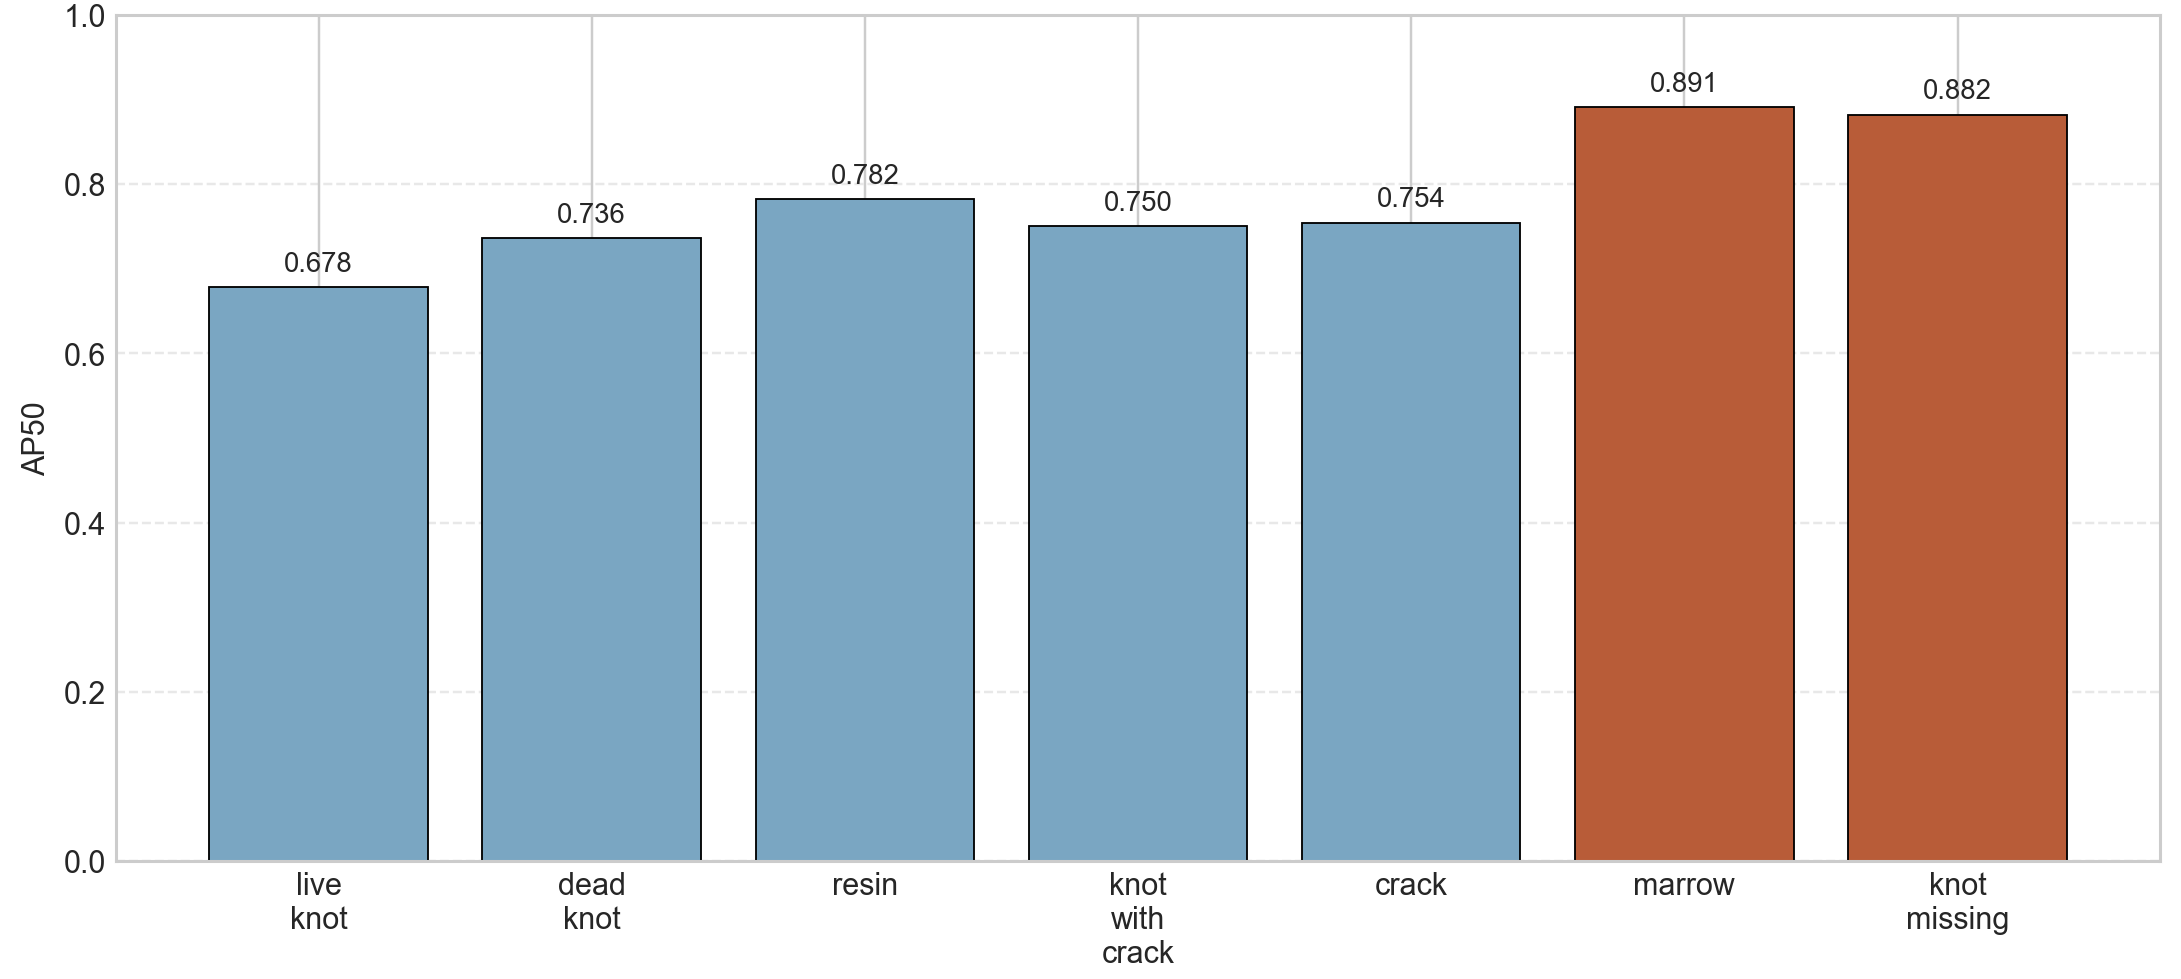
\includegraphics[width=0.90\linewidth]{figures/y0_3600_classwise_ap50_1.png}
  \caption{Class-wise AP50 of \texttt{Y0-3600e200}}
  \label{fig:y0-classwise-ap50}
\end{figure}

Figure~\ref{fig:yolo-progress} shows the training dynamics of the 200-epoch YOLOv8s run on the curated benchmark. AP50 rises quickly during the early schedule, reaches its peak at epoch 55, and then stays in a stable high-performance regime through the remainder of training. The loss curves also become progressively smoother over the schedule, which supports using this run as the final literature-facing compact baseline.

\begin{figure*}[t]
  \centering
  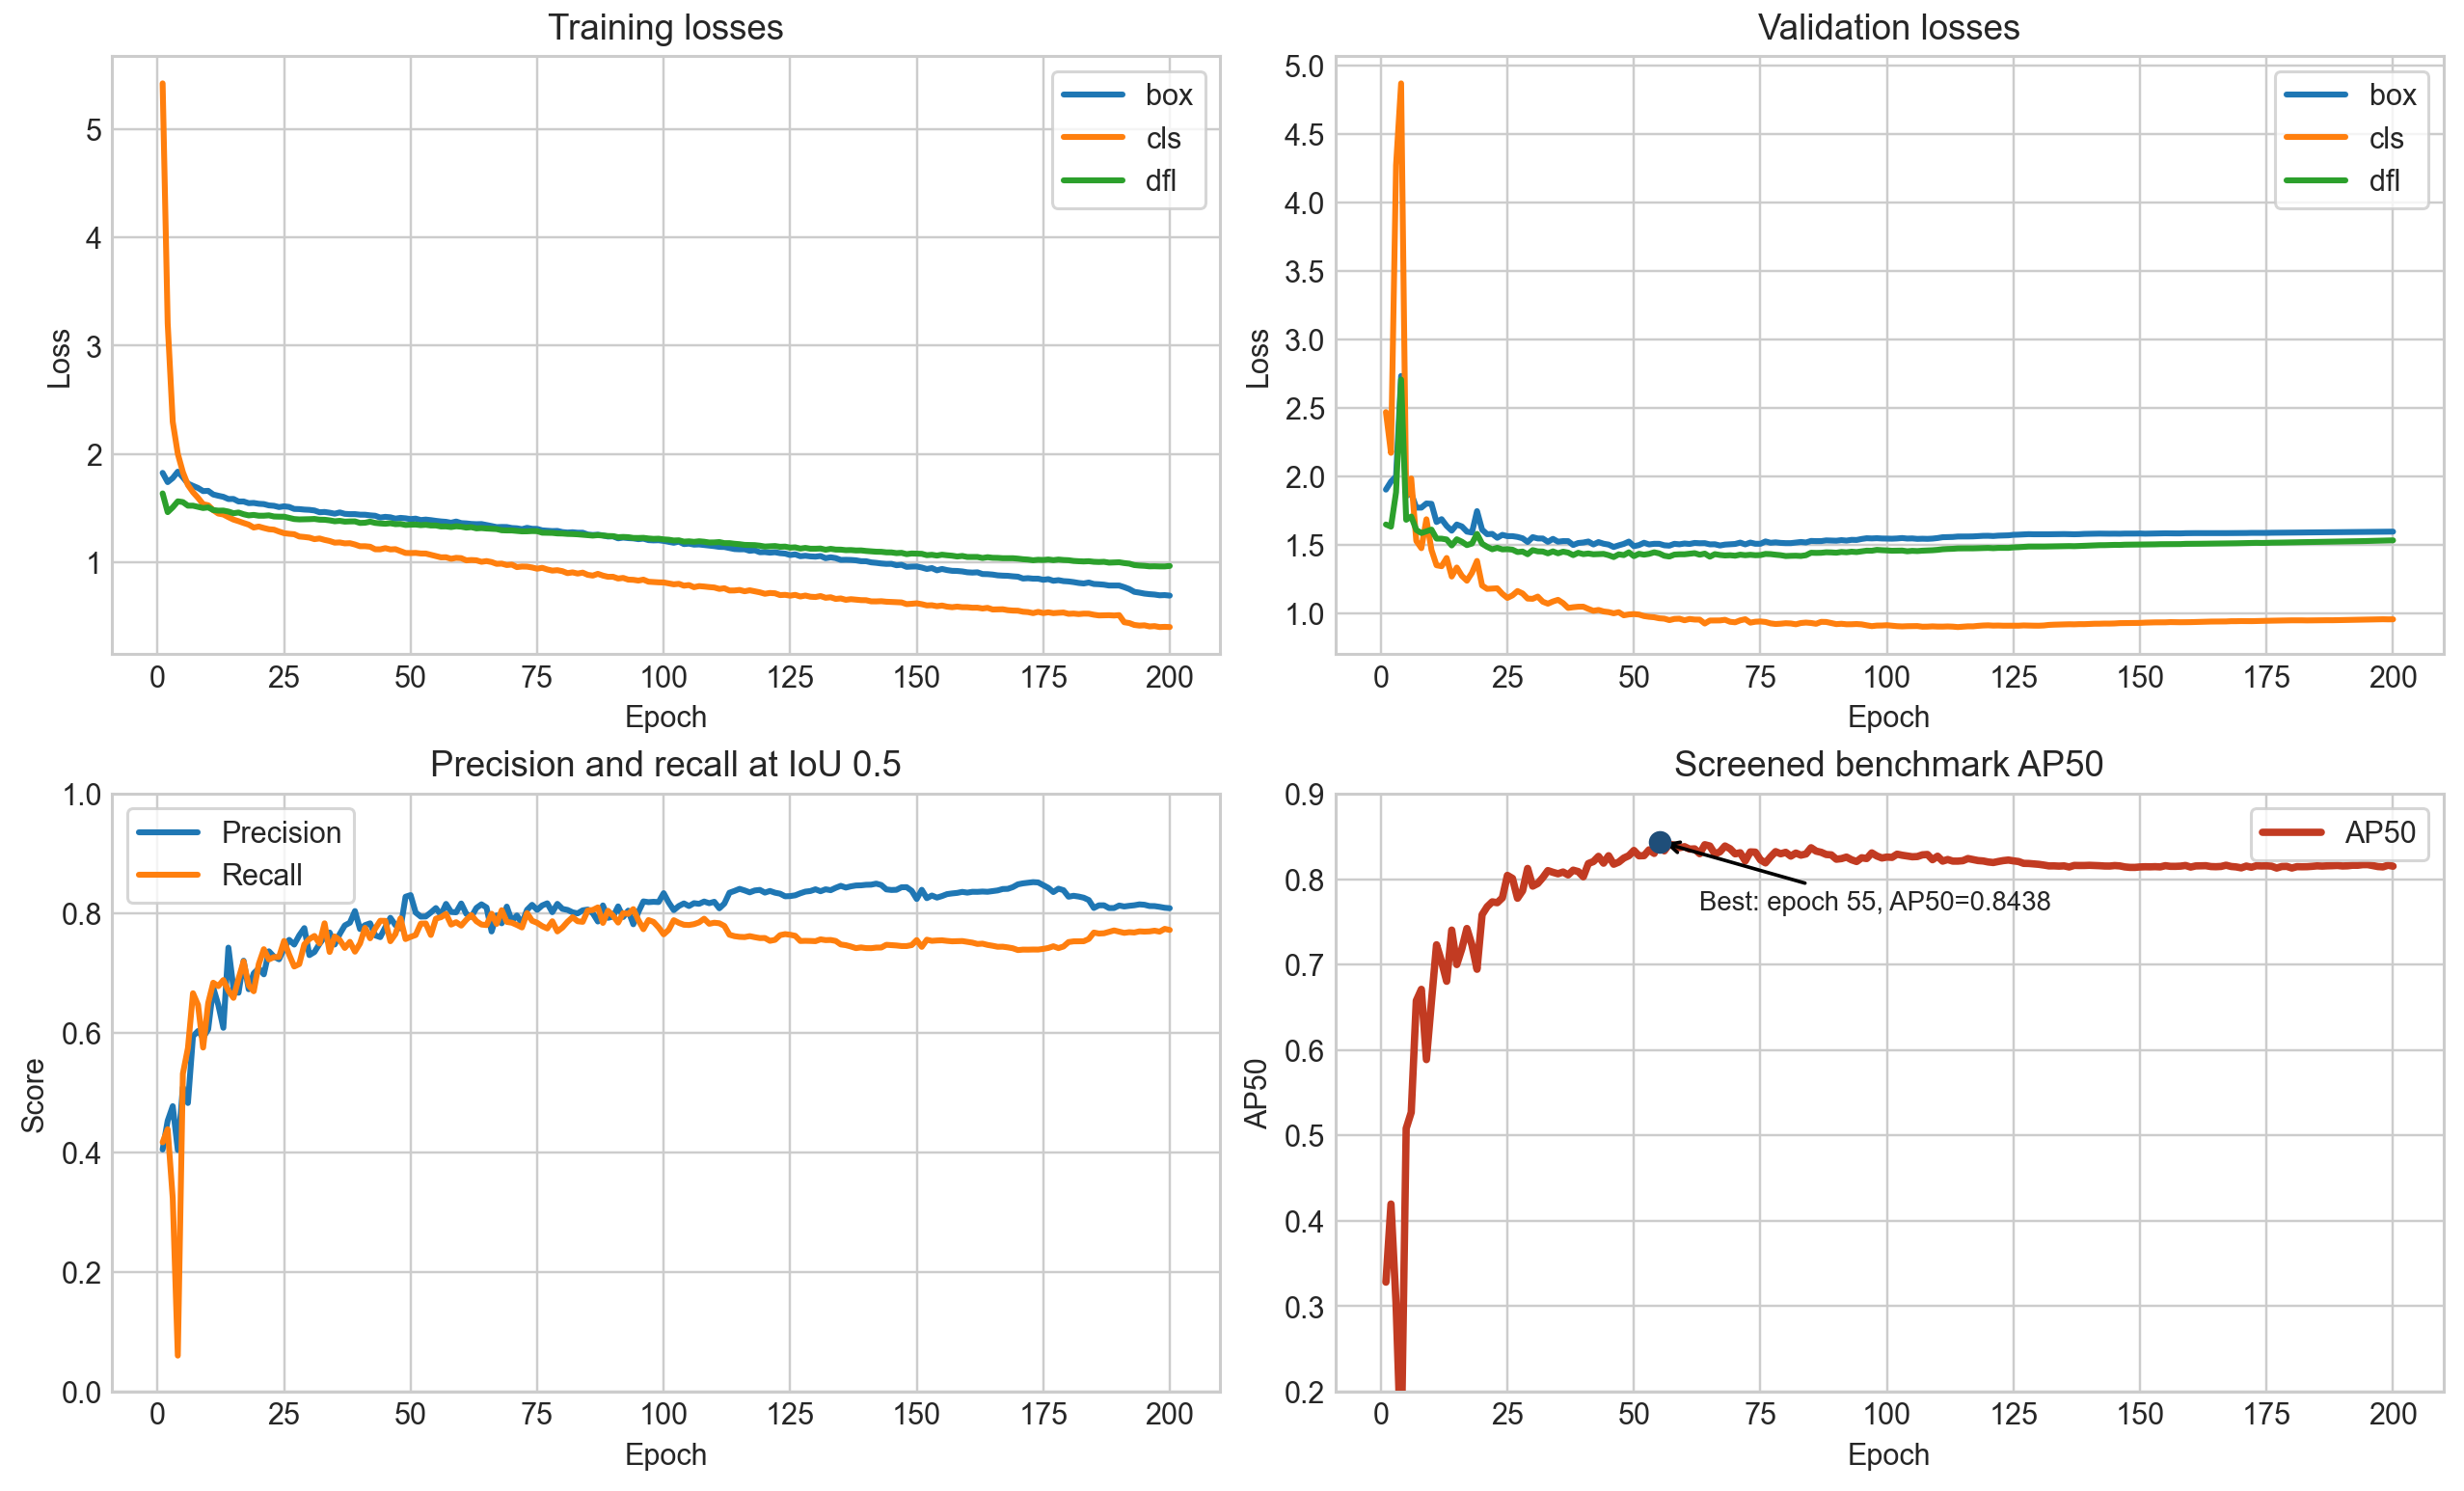
\includegraphics[width=0.92\linewidth]{figures/yolo_protocol_progress_1.png}
  \caption{Training progress of the 200-epoch YOLOv8s run on the curated benchmark. The model reaches its best AP50 at epoch 55 and then stays in a stable high-performance regime, which supports using this run for literature-facing comparison.}
  \label{fig:yolo-progress}
\end{figure*}

\subsection{Target-Domain Adaptation Results on VNWoodKnot}
\label{sec:external-results}

Table~\ref{tab:external} summarizes a representative single-seed target-domain adaptation comparison on VNWoodKnot. The held-out target-domain test split used for this comparison contains 229 images, 155 target boxes, and 75 negative \texttt{knot\_free} images. Under the seed-42 run shown here, three observations are notable:

\begin{itemize}[leftmargin=1.5em]
  \item On the held-out target-domain test split in this representative run, \texttt{T1} reaches 0.8312 AP50, whereas \texttt{T0} reaches 0.7753. This is a gain of 5.59 AP50 points under the same 50-epoch adaptation budget.
  \item \texttt{T1} is also cleaner: precision improves from 0.5370 to 0.6730 while recall improves from 0.8903 to 0.9161, and the total number of predictions drops from 257 to 211.
  \item The validation trajectories still show an optimization advantage for source initialization. \texttt{T1} reaches 0.70 AP50 by epoch 9 and 0.80 by epoch 31, whereas \texttt{T0} reaches the same thresholds only at epochs 19 and 40, respectively.
\end{itemize}

These seed-42 results indicate that the target task is learnable within a modest training budget and that the curated-benchmark source checkpoint can produce a strong transferred run under one representative initialization. At the same time, this single-run view is not taken as the final robustness claim of the paper. The repeated-seed analysis below is therefore essential: it separates one encouraging transferred run from the broader question of whether the held-out target-domain advantage persists across seeds.

\begin{table}[t]
  \centering
  \caption{Single-seed target-domain adaptation on VNWoodKnot under a fixed 50-epoch budget. Results are reported on the held-out target-domain test split (229 images, 155 target boxes, 75 negative \texttt{knot\_free} images) using the best checkpoint selected within each 50-epoch run.}
  \label{tab:external}
  \footnotesize
  \setlength{\tabcolsep}{4pt}
  \begin{tabularx}{\linewidth}{>{\raggedright\arraybackslash}p{0.10\linewidth} >{\raggedright\arraybackslash}p{0.23\linewidth} c c c X}
    \toprule
    ID & Setting & AP50 & Prec.50 & Rec.50 & Notes \\
    \midrule
    \texttt{T0} & target-only supervised training & 0.7753 & 0.5370 & 0.8903 & held-out test (229 images, 155 targets), seed 42, 257 predictions \\
    \texttt{T1} & \texttt{Y0-3600e200} $\rightarrow$ fine-tune & \best{0.8312} & \best{0.6730} & \best{0.9161} & held-out test (229 images, 155 targets), seed 42, 211 predictions \\
    \bottomrule
  \end{tabularx}
\end{table}

Figure~\ref{fig:vnwoodknot-transfer} visualizes this seed-42 comparison. The left panel shows held-out test AP50 overall and by class. Under this single run, the largest gain comes from \texttt{live\_knot}, where AP50 rises from 0.7106 to 0.8324. For \texttt{dead\_knot}, AP50 stays nearly unchanged, but precision and recall still improve. The right panel shows the first 50 validation epochs and confirms that \texttt{T1} enters a useful accuracy regime much earlier than \texttt{T0}. These views therefore illustrate the motivation for transfer under one representative run, while the repeated-seed validation and held-out-test analyses below assess how much of that advantage persists across repeated initializations.

\begin{figure}[t]
  \centering
  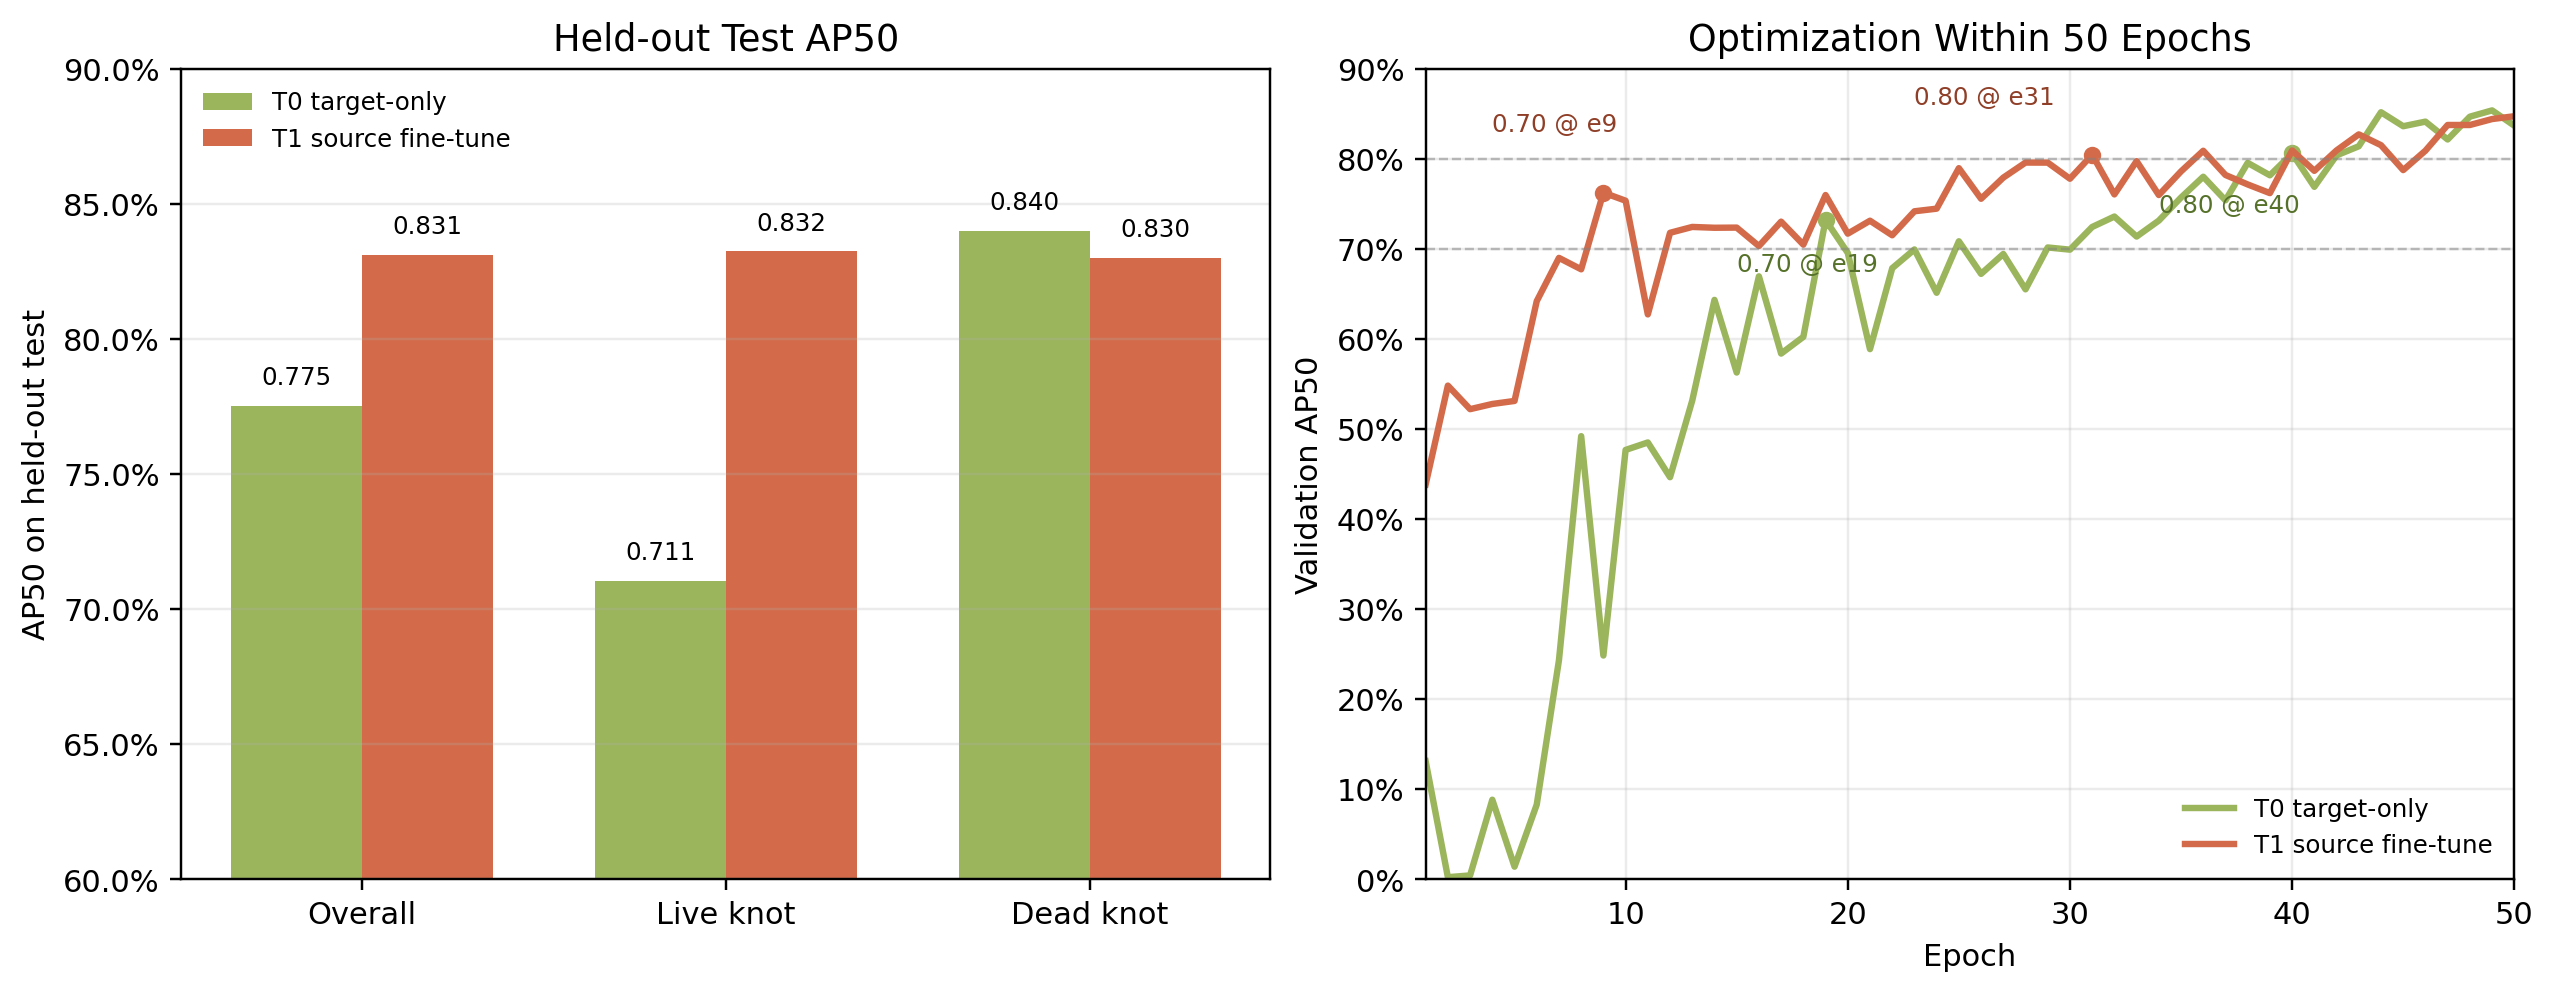
\includegraphics[width=0.98\linewidth]{figures/vnwoodknot_adaptation_50e.png}
  \caption{VNWoodKnot adaptation under a fixed 50-epoch budget. Left: held-out test AP50 overall and by class for target-only training and curated-benchmark source fine-tuning. Right: validation AP50 trajectories for the first 50 epochs.}
  \label{fig:vnwoodknot-transfer}
\end{figure}

\subsection{Multi-Seed Robustness Evaluation}
\label{sec:multiseed-results}

To assess robustness with respect to random initialization, the main text keeps only a short repeated-seed summary, while Appendix~\ref{sec:appendix-robustness} collects the fuller 50-epoch robustness tables. Table~\ref{tab:multiseed-current} reports mean $\pm$ standard deviation over seeds 42, 43, 44, and 45 for the validation-side target-domain adaptation runs, and Table~\ref{tab:multiseed-transfer-test} reports the corresponding held-out-test aggregates.

Under the shared 50-epoch budget, the repeated-seed in-domain ablations do not overturn the compact-baseline ranking. In native YOLO validation, \texttt{Y0} remains highest at $0.8379 \pm 0.0050$ AP50, \texttt{Y2} tracks closely at $0.8355 \pm 0.0033$, and \texttt{Y1} reaches $0.8299 \pm 0.0082$. Under the shared repo evaluator on the held-out curated test split, the ordering becomes \texttt{Y0} ($0.7791 \pm 0.0052$) $>$ \texttt{Y1} ($0.7757 \pm 0.0084$) $>$ \texttt{Y2} ($0.7725 \pm 0.0042$), so none of the local YOLO refinements yields a robust short-budget test-time AP50 gain over the compact baseline. For VNWoodKnot, the validation repeats still favor source initialization slightly: \texttt{T1} reaches $0.8535 \pm 0.0101$ AP50 versus $0.8444 \pm 0.0088$ for \texttt{T0}, and it also retains the higher mean precision. The held-out-test aggregates in Table~\ref{tab:multiseed-transfer-test}, however, favor \texttt{T0}: target-only training reaches $0.7909 \pm 0.0136$ AP50, whereas source-initialized fine-tuning reaches $0.7730 \pm 0.0409$. Under the present 50-epoch setting, transfer therefore changes optimization behavior and the precision--recall trade-off, but it does not yield a robust held-out-test AP50 gain across seeds.

\begin{table*}[t]
  \centering
  \caption{Validation-side multi-seed robustness for target-domain adaptation under the 50-epoch setting. Reported values are mean $\pm$ standard deviation over seeds 42, 43, 44, and 45.}
  \label{tab:multiseed-current}
  \scriptsize
  \setlength{\tabcolsep}{4pt}
  \begin{tabularx}{\textwidth}{>{\raggedright\arraybackslash}p{0.28\textwidth} >{\raggedright\arraybackslash}p{0.16\textwidth} >{\raggedright\arraybackslash}p{0.16\textwidth} >{\raggedright\arraybackslash}p{0.16\textwidth} X}
    \toprule
    Setting & Split & AP50 & Prec.50 & Rec.50 \\
    \midrule
    \texttt{T0} (target-only) & VNWoodKnot val & $0.844 \pm 0.009$ & $0.762 \pm 0.037$ & $0.820 \pm 0.043$ \\
    \texttt{T1} (\texttt{Y0-3600e200} $\rightarrow$ fine-tune) & VNWoodKnot val & $0.854 \pm 0.010$ & $0.798 \pm 0.024$ & $0.819 \pm 0.011$ \\
    \bottomrule
  \end{tabularx}
\end{table*}

\begin{table}[t]
  \centering
  \caption{Held-out-test multi-seed robustness for target-domain adaptation on VNWoodKnot. All rows correspond to 50-epoch runs, and reported values are mean $\pm$ standard deviation over seeds 42, 43, 44, and 45.}
  \label{tab:multiseed-transfer-test}
  \footnotesize
  \setlength{\tabcolsep}{4pt}
  \begin{tabularx}{\linewidth}{>{\raggedright\arraybackslash}p{0.30\linewidth} >{\raggedright\arraybackslash}p{0.16\linewidth} >{\raggedright\arraybackslash}p{0.16\linewidth} X}
    \toprule
    Setting & AP50 & Prec.50 & Rec.50 \\
    \midrule
    \texttt{T0} (target-only) & $0.791 \pm 0.014$ & $0.539 \pm 0.027$ & $0.916 \pm 0.017$ \\
    \texttt{T1} (\texttt{Y0-3600e200} $\rightarrow$ fine-tune) & $0.773 \pm 0.041$ & $0.599 \pm 0.074$ & $0.869 \pm 0.032$ \\
    \bottomrule
  \end{tabularx}
\end{table}

\subsection{Inference Computational Cost}
\label{sec:efficiency-results}

Because practical deployment is one of the main motivations of this study, we also profile inference cost for the detector families and transfer settings reported in the final comparison. Table~\ref{tab:efficiency} reports parameter count, FLOPs, latency, throughput, and peak inference memory for a single-image batch at image size $1024$ under the same profiling environment.

The compact YOLOv8s baseline remains attractive from a deployment perspective: despite higher FLOPs than the MobileNet baselines, it runs faster and uses less peak inference memory in the present environment. The P2-head variant (\texttt{Y1-e200}) is the only YOLO refinement that clearly increases inference cost, raising parameters, FLOPs, latency, and memory without improving AP50 over \texttt{Y0-3600e200}. By contrast, the WNIoU-style branch (\texttt{Y2-e200}) keeps essentially the same inference footprint as the YOLO baseline, which is consistent with its role as a loss-level training change rather than an architectural modification. The same logic applies to \texttt{T0} and \texttt{T1}: source initialization changes the starting weights but not the deployed model structure, so their parameter count, FLOPs, and memory remain effectively identical, and the small latency gap between them should not be read as a structural cost difference.

\begin{table}[t]
  \centering
  \caption{Inference computational cost of the detector families and transfer settings reported in the main text at image size $1024$ and batch size $1$.}
  \label{tab:efficiency}
  \footnotesize
  \setlength{\tabcolsep}{4pt}
  \begin{tabularx}{\linewidth}{>{\raggedright\arraybackslash}p{0.29\linewidth} c c c c c}
    \toprule
    Model & Params (M) & FLOPs (G) & Latency (ms) & Throughput (img/s) & Peak Mem. (GB) \\
    \midrule
    Low-capacity MobileNet baseline & 18.99 & 19.64 & 9.55 & 104.70 & 0.257 \\
    High-resolution MobileNet baseline & 18.99 & 43.33 & 12.96 & 77.14 & 0.257 \\
    \texttt{Y0-3600e200} & 9.84 & 60.38 & 7.48 & 133.69 & 0.154 \\
    \texttt{Y1-e200} & 10.03 & 81.24 & 9.06 & 110.39 & 0.230 \\
    \texttt{Y2-e200} & 9.84 & 60.38 & 7.23 & 138.22 & 0.154 \\
    \texttt{T0} & 9.84 & 60.36 & 5.98 & 167.23 & 0.154 \\
    \texttt{T1} & 9.84 & 60.36 & 7.59 & 131.79 & 0.154 \\
    \bottomrule
  \end{tabularx}
\end{table}

\section{Discussion}
\label{sec:discussion}

The strongest result in the evaluated design space still comes from the compact YOLOv8s baseline. The long-schedule run on the curated benchmark places the model toward the upper end of the range reported in the closest public papers built on the same public benchmark domain. That matters because the gain does not come from a heavier detector or an extra architectural block. We still stop short of a blanket SOTA claim: the reconstructed benchmark, checkpoint policy, and evaluation details are not identical across studies. Even with that caveat, the curated-benchmark YOLO result is strong enough to support a direct public-facing comparison.

The two-stage MobileNet branch serves mainly as a reference rather than as the top model. It provides a lightweight proposal-based comparison and stays reasonably competitive, especially on the broader full protocol. Even so, it does not catch the compact YOLO baseline. The same is true for the local YOLO changes examined here. Under the repeated-seed 50-epoch checks, none of the internal YOLO variants produces a robust held-out-test AP50 gain over the compact baseline, even though \texttt{Y2} tracks it closely in native validation and \texttt{Y1} remains competitive. The matched 200-epoch reruns keep the same overall ranking. For this dataset and training recipe, model family mattered more than either of those local edits.

Within the present training budgets and evaluation setup, protocol choice changes the picture enough that it cannot be treated as a reporting detail. The full seven-class protocol stays below the curated benchmark even after the extra 200-epoch rerun, and the result does not show a gain for the longer full-protocol run. The VNWoodKnot experiment points in the same direction, but with a more nuanced message. Source initialization helps optimization and slightly improves the mean validation metrics across four seeds, yet the same advantage does not survive as a robust held-out-test AP50 gain under the current 50-epoch budget: the four-seed test aggregate favors \texttt{T0}, and \texttt{T1} is more variable across seeds. The practical bottleneck is therefore not just finding a source checkpoint that can produce one strong transferred run. It is establishing an adaptation recipe whose held-out-test behavior remains stable when the protocol broadens or when the data source changes.

The ablation results indicate that, under the present dataset, label space, and training recipe, the missing ingredient is not simply a higher-resolution head or a different box-loss term. The P2-head branch remains slightly below the compact baseline on AP50 under both short and long schedules, even though it stays competitive on mAP50--95. The WNIoU-style long-schedule rerun comes closer, but still does not overturn the baseline ranking. Those ideas may help elsewhere, but here they were not enough on their own.

This study has several limitations. The broader full-protocol and external adaptation results are still restricted to relatively short target-domain budgets, and the paper does not yet report matched training-time or energy measurements across schedules and detector families. In addition, the full reproducibility bundle is described here but not embedded directly in the manuscript. Those details narrow the scope of the claims and should be tightened in a final journal version.

\section{Conclusion}
\label{sec:conclusion}

This study examined how detector-family choice, protocol breadth, and source-to-target transfer affect wood surface defect detection across a public benchmark domain and a low-resource target domain.

The strongest curated-benchmark result in the evaluated design space comes from the compact YOLOv8s baseline. Within the 50-epoch reference setting, YOLOv8s remained ahead of the tested MobileNet-based references, and the repeated-seed short-budget checks do not overturn that ranking once held-out-test AP50 is considered. The matched 200-epoch reruns keep the same ordering on the curated benchmark: \texttt{Y1-e200} reaches 83.70\% AP50 and \texttt{Y2-e200} reaches 83.93\% AP50, both below the 84.38\% AP50 of \texttt{Y0-3600e200}. On the broader full seven-class protocol, the 50-epoch reference reaches 80.39\% AP50, while the 200-epoch rerun raises native YOLO AP50 only slightly to 81.16\% and does not remove the broader-protocol gap. In this study, detector-family choice mattered more than the tested local refinements, and protocol breadth changed the apparent difficulty of the task.

The external evaluation showed the same sensitivity from another angle. Strong in-domain results did not remove the need for target-domain adaptation, but they also did not translate into a uniformly positive transfer result. Under a fixed 50-epoch budget on VNWoodKnot, the representative seed-42 run favored source-initialized fine-tuning, and the four-seed validation averages remain slightly higher for \texttt{T1}. The repeated-seed held-out test aggregate, however, does not confirm a robust AP50 advantage over target-only training: \texttt{T0} averages 79.09\% AP50, whereas \texttt{T1} averages 77.30\%. The target task is learnable, and transfer remains worth studying, but the present evidence supports a nuanced conclusion about robustness rather than a blanket claim that source initialization always helps.

Future work will focus on extending target-domain adaptation beyond the present 50-epoch budget, adding matched training-time benchmarking across schedules, and studying transfer-aware adaptation strategies on VNWoodKnot.

\appendix
\section{Supplementary Robustness Tables}
\label{sec:appendix-robustness}

This appendix collects the repeated-seed details that are useful for reproducibility but would otherwise diffuse the main text. The main text therefore keeps only the condensed robustness conclusions, while the tables below report the corresponding 50-epoch AP50 matrices.

\begin{table*}[t]
  \centering
  \caption{Fifty-epoch repeated-seed in-domain YOLO summary on the curated benchmark. Native validation AP50 comes from the best-checkpoint Ultralytics training logs, whereas held-out test metrics come from the shared repo evaluator. All values are mean $\pm$ standard deviation over seeds 42, 43, 44, and 45.}
  \label{tab:app-curated-summary}
  \footnotesize
  \setlength{\tabcolsep}{4pt}
  \begin{tabularx}{\textwidth}{>{\raggedright\arraybackslash}p{0.22\textwidth} c c c c}
    \toprule
    Setting & Native val AP50 & Held-out test AP50 & Test Prec.50 & Test Rec.50 \\
    \midrule
    \texttt{Y0} (YOLOv8s baseline) & $0.8379 \pm 0.0050$ & $0.7791 \pm 0.0052$ & $0.5491 \pm 0.0118$ & $0.8540 \pm 0.0111$ \\
    \texttt{Y1} (P2 head) & $0.8299 \pm 0.0082$ & $0.7757 \pm 0.0084$ & $0.5375 \pm 0.0051$ & $0.8587 \pm 0.0072$ \\
    \texttt{Y2} (WNIoU-style loss) & $0.8355 \pm 0.0033$ & $0.7725 \pm 0.0042$ & $0.5484 \pm 0.0048$ & $0.8523 \pm 0.0047$ \\
    \bottomrule
  \end{tabularx}
\end{table*}

\begin{table*}[t]
  \centering
  \caption{Per-seed AP50 detail for the 50-epoch in-domain YOLO checks on the curated benchmark.}
  \label{tab:app-curated-perseed}
  \scriptsize
  \setlength{\tabcolsep}{4pt}
  \begin{tabularx}{\textwidth}{>{\raggedright\arraybackslash}p{0.26\textwidth} c c c c X}
    \toprule
    Setting / Split & Seed 42 & Seed 43 & Seed 44 & Seed 45 & Mean $\pm$ std \\
    \midrule
    \texttt{Y0} native val & 0.83569 & 0.83207 & 0.84326 & 0.84059 & $0.8379 \pm 0.0050$ \\
    \texttt{Y1} native val & 0.82594 & 0.82313 & 0.84175 & 0.82889 & $0.8299 \pm 0.0082$ \\
    \texttt{Y2} native val & 0.83057 & 0.83803 & 0.83660 & 0.83670 & $0.8355 \pm 0.0033$ \\
    \texttt{Y0} held-out test & 0.78436 & 0.77248 & 0.78163 & 0.77778 & $0.7791 \pm 0.0052$ \\
    \texttt{Y1} held-out test & 0.78389 & 0.77715 & 0.76390 & 0.77777 & $0.7757 \pm 0.0084$ \\
    \texttt{Y2} held-out test & 0.77147 & 0.77870 & 0.77019 & 0.76944 & $0.7725 \pm 0.0042$ \\
    \bottomrule
  \end{tabularx}
\end{table*}

\begin{table*}[t]
  \centering
  \caption{Per-seed AP50 detail for the 50-epoch target-domain adaptation runs on VNWoodKnot. Validation AP50 comes from the native YOLO training logs, and held-out test AP50 comes from the shared repo evaluator.}
  \label{tab:app-transfer-perseed}
  \scriptsize
  \setlength{\tabcolsep}{4pt}
  \begin{tabularx}{\textwidth}{>{\raggedright\arraybackslash}p{0.28\textwidth} c c c c X}
    \toprule
    Setting / Split & Seed 42 & Seed 43 & Seed 44 & Seed 45 & Mean $\pm$ std \\
    \midrule
    \texttt{T0} validation & 0.85368 & 0.83294 & 0.84817 & 0.84269 & $0.8444 \pm 0.0088$ \\
    \texttt{T1} validation & 0.84720 & 0.85164 & 0.84687 & 0.86838 & $0.8535 \pm 0.0101$ \\
    \texttt{T0} held-out test & 0.77532 & 0.78900 & 0.79072 & 0.80843 & $0.7909 \pm 0.0136$ \\
    \texttt{T1} held-out test & 0.83119 & 0.75545 & 0.76839 & 0.73704 & $0.7730 \pm 0.0409$ \\
    \bottomrule
  \end{tabularx}
\end{table*}

\section*{Funding Statement}
The author received no specific funding for this study.

\section*{Acknowledgment}
Not applicable.

\section*{Author Contributions}
Khanh Nguyen-Trong conceived the study, designed the methodology, implemented the code, ran the experiments, analyzed the results, and wrote the manuscript.

\section*{Availability of Data and Materials}
This study is based on experiment outputs and scripts stored in the study repository. Upon acceptance, we plan to release the training scripts, evaluation scripts, benchmark-construction utilities, split manifests, the list of selected 3,600 source images used to define the curated benchmark, evaluator settings, paper tables, and representative training curves used to generate the reported results. Redistribution of raw image data and derived manifests will remain subject to the licenses and access conditions of the original datasets.

\section*{Ethics Approval}
Not applicable.

\section*{Conflicts of Interest}
The authors declare that they have no conflicts of interest to report regarding the present study.

\bibliographystyle{unsrtnat}
\bibliography{references}

\end{document}
